\subsection{$\alpha = 1$, unary}

Let the point where the first transcript bead was fixed be $p$ and let $n=|\mathrm{seed}|+1$. We will argue about the situation when the first bead is stabilized outside $\hexagon_p^n$ (a hexagon of radius $n$). Let this be the $i$th bead of the transcript. Without loss of generality, we can translate the origin $(0,0)$ to the coordinates of bead $i-1$ (which is still in $\hexagon_p^n$), and we can assume that the bead outside the hexagon is fixed at $(1,1)$ (see Fig.~\ref{fig:hexagonOut}).
\begin{figure}
	\centering
	\includegraphics[width=0.3\linewidth]{./Fig/hexagonOut}
	\caption{$N_p^n$ and the position $(1,1)$ of the first bead fixed outside of it.}
	\label{fig:hexagonOut}
\end{figure}

In the elongation that places bead $i$ at $(1,1)$ there are two possibilities:
\begin{itemize}
	\item $i$ forms a bond with a bead at $(1,0)$.
	\item  $i$ does not bond to anything and $i+1$ is at $(2,1)$ bonding with a bead at $(2,0)$. If there is no bead at $(1,0)$, then placing $i$ at $(1,0)$ instead of $(1,1)$ results in the same number of bonds, leading to nondeterminism. Therefore, there has to be a bead at $(1,0)$ and it is inert, otherwise it would bond to $i$. This is analogous to case 1. below.%as in Fig.~\ref{fig:hexagonOut1}.
	\begin{figure}
		\centering
		\includegraphics[width=0.2\linewidth]{./Fig/hexagonOut1}
		%\caption{}
		\label{fig:hexagonOut1}
	\end{figure}
	
\end{itemize}
 
%The only position with which $(1,1)$ can form a bond is $(1,0)$. This means that there is a bead at $(1,0)$, which bonds to bead $i$, otherwise there are other conformations in which beads $i$ and $i+1$ add one bond to the conformation, making the behavior nondeterministic.

The next bead, $i+1$, can be fixed at $(2,1)$ or at $(0,1)$ as all other possibilities result in nondeterministic behavior immediately, so we have two cases.

\begin{enumerate}
	\item bead $i+1$ is fixed at $(2,1)$ and can bond with a bead at $(2,0)$. Now consider bead $i+2$. For $i+1$ to be fixed at $(2,1)$, $i+2$ needs to form a bond somewhere, otherwise $i+2$ could go to $(2,1)$ forming the bond with the bead at $(2,0)$ and there would be two conformations with the maximal $1$ bond. The only possibility is that there is a bead at $(3,0)$ and $i+2$ can bond with it when placed at $(3,1)$. We can apply the same argument inductively: there is some $m\geq 0$ such that grid points $(\ell,0)$ are occupied by active beads, for all $\ell\in \{2,\dots,2+m\}$, and there is no bead at $(3+m,0)$. Such an $m$ exists, and it is not greater than $n$. Then, bead $i+\ell$ is fixed at $(\ell+1,1)$ and bonds with $(\ell+1,0)$. However, bead $i+2+m$ cannot be fixed anywhere, because $i+2+m$ and $i+3+m$ can only add one bond to the conformation, and that is possible either with $i+2+m \rightarrow (2+m,1)$, $i+3+m \rightarrow (3+m,1)$ or with $i+2+m \rightarrow (2+m,2)$, $i+3+m \rightarrow (2+m,1)$. 
	\begin{figure}
		\centering
		\includegraphics[width=0.6\linewidth]{./Fig/hexagonOut2}
		\caption{}
		\label{fig:hexagonout2}
	\end{figure}
	
	\item bead $i+1$ is fixed at $(0,1)$. This is only possible if
	\begin{enumerate}
		\item there is an inactive bead at $(-1,0)$ and an active one at $(-2,0)$. This case is symmetrical to (1).
		\item there is no bead at $(-1,0)$, bead $i+1$ can bond with bead $i-1$ at $(0,0)$ and the bead $i+2$ can be placed at $(-1,0)$ where it can bond with $(-2,0)$, $(-2,-1)$ or $(-1,-1)$. This leads to nondeterminism, because bead $i$ at $(-1,0)$ and bead $i+1$ at $(0,1)$ has two bonds, just as the original conformation.
		\item there is a bead at $(-1,0)$ and bead $i+1$ can bond with that or with bead $i-1$ at $(0,0)$. However, this means that placing bead $i$ at $(0,1)$ at bead $i+1$ at $(1,1)$ creates the same number of hydrogen bonds, thus resulting in bead $i$ not being placed deterministically.
		
	\end{enumerate}
\end{enumerate}




\begin{figure}
	\centering
	%\includegraphics[width=0.3\linewidth]{./hexagonOut1}
	%\hspace{10mm} %
	\includegraphics[width=0.6\linewidth]{./Fig/hexagonOut3}
	
	\caption{}
	\label{fig:hexagonOut2}
\end{figure}


\subsection{In the case of $\delta = 3$}

We discuss when the length of seed is $n$. If the length of seed is $n$, the seed will be in an equilateral hexagon with a radius of $n$ when it is given. We will begin our disscussion by considering the moment when a first bead is fixed on a side of an equilateral hexagon with a radius of $n+1$. Let us assume that a fixed bead on a side of an equilateral hexagon with a radius of $n$ is able to make a hydrogen bond. If it is able to make only two hydrogen bonds, it will be nondeterministic because there are two possibilities that it makes two structures in Fig.5. Therefore, it needs to make three hydrogen bonds to determine the only structure.\\

\begin{figure}
  \begin{center}
  \begin{tabular}{cc}
    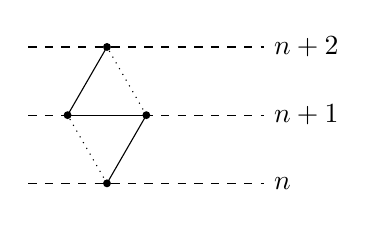
\begin{tikzpicture}
      \draw [dashed] (-1.0, 0.0) -- (2.0, 0.0);
      \fill (2.0, 0.0) node [right] {$n$};
      \draw [dashed] (-1.0, 0.866) -- (2.0, 0.866);
      \fill (2.0, 0.866) node [right] {$n+1$};
      \draw [dashed] (-1.0, 1.732) -- (2.0, 1.732);
      \fill (2.0, 1.732) node [right] {$n+2$};
      \fill (0,0) circle [radius = 0.05];
      \begin{scope}[shift = (0 : 0.0)]
        \foreach \theta in {60, 120}{
          \fill (0,0) [transform canvas = {shift = (\theta : 1.0)}] circle [radius = 0.05];
        }
        \draw (0 : 0.0) -- (60 : 1.0);
        \draw (60 : 1.0) -- (120 : 1.0);
        \draw [dotted] (0 : 0.0) -- (120 : 1.0);
      \end{scope}
      \begin{scope}[shift = (60 : 1.0)]
        \draw [dotted] (0 : 0.0) -- (120 : 1.0);
      \end{scope}
      \begin{scope}[shift = (120 : 1.0)]
        \foreach \theta in {60}{
        \fill (0,0) [transform canvas = {shift = (\theta : 1.0)}] circle [radius = 0.05];
        }
        \draw (0 : 0.0) -- (60 : 1.0);
      \end{scope}
    \end{tikzpicture}

    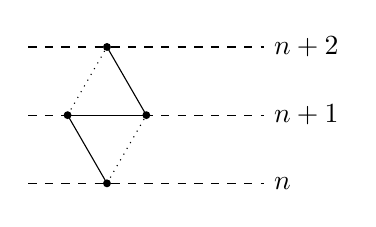
\begin{tikzpicture}
      \draw [dashed] (-1.0, 0.0) -- (2.0, 0.0);
      \fill (2.0, 0.0) node [right] {$n$};
      \draw [dashed] (-1.0, 0.866) -- (2.0, 0.866);
      \fill (2.0, 0.866) node [right] {$n+1$};
      \draw [dashed] (-1.0, 1.732) -- (2.0, 1.732);
      \fill (2.0, 1.732) node [right] {$n+2$};
      \fill (0,0) circle [radius = 0.05];
      \begin{scope}[shift = (0 : 0.0)]
        \foreach \theta in {60, 120}{
          \fill (0,0) [transform canvas = {shift = (\theta : 1.0)}] circle [radius = 0.05];
        }
        \draw [dotted] (0 : 0.0) -- (60 : 1.0);
        \draw (60 : 1.0) -- (120 : 1.0);
        \draw (0 : 0.0) -- (120 : 1.0);
      \end{scope}
      \begin{scope}[shift = (60 : 1.0)]
        \draw (0 : 0.0) -- (120 : 1.0);
      \end{scope}
      \begin{scope}[shift = (120 : 1.0)]
        \foreach \theta in {60}{
        \fill (0,0) [transform canvas = {shift = (\theta : 1.0)}] circle [radius = 0.05];
        }
        \draw [dotted](0 : 0.0) -- (60 : 1.0);
      \end{scope}
    \end{tikzpicture}
    \end{tabular}
    \caption{}
  \end{center}
\end{figure}

There are the two cases in which a first bead is fixed on a side of an equilateral hexagon with a radius of $n+1$ and it makes three hydrogen bonds in Fig.6. If it makes three hydrogen bonds once such as Fig6., it will make three hyrogen bonds forever to be deterministic. This becomes nondeterministic finally, such as in Fig.7., when it reaches a corner of an equilateral hexagon. Thus, the fixed bead on a side of an equilateral hexagon with a radius of $n$ has to make a hydrogen bond with a bead in an equilateral hexagon.

\begin{figure}
  \begin{center}
  \begin{tabular}{cc}
    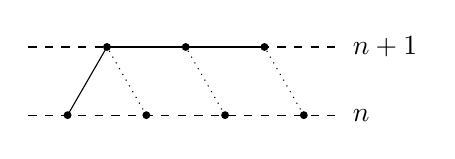
\begin{tikzpicture}
      \draw [dashed] (-0.5, 0.0) -- (3.5, 0.0);
      \fill (3.5, 0.0) node [right] {$n$};
      \draw [dashed] (-0.5, 0.866) -- (3.5, 0.866);
      \fill (3.5, 0.866) node [right] {$n+1$};
      \fill (0,0) circle [radius = 0.05];
      \begin{scope}[shift = (0 : 0.0)]
        \foreach \theta in {0, 60}{
          \fill (0,0) [transform canvas = {shift = (\theta : 1.0)}] circle [radius = 0.05];
        }
        \draw (0 : 0.0) -- (60 : 1.0);
      \end{scope}
      \begin{scope}[shift = (0 : 2.0)]
        \fill (0,0) circle [radius = 0.05];
        \foreach \theta in {0, 60, 120}{
          \fill (0,0) [transform canvas = {shift = (\theta : 1.0)}] circle [radius = 0.05];
        }
        \draw [dotted] (0 : 0.0) -- (120 : 1.0);
      \end{scope}
      \begin{scope}[shift = (60 : 1.0)]
          \draw (0 : 0.0) -- (0 : 2.0);
      \end{scope}
      \begin{scope}[shift = (0 : 1.0)]
          \draw [dotted] (0 : 0.0) -- (120 : 1.0);
      \end{scope}
      \begin{scope}[shift = (0 : 3.0)]
          \draw [dotted] (0 : 0.0) -- (120 : 1.0);
      \end{scope}
    \end{tikzpicture}

    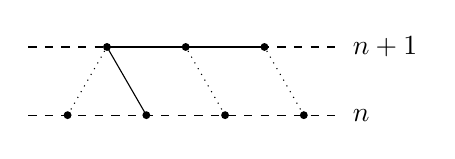
\begin{tikzpicture}
      \draw [dashed] (-1.5, 0.0) -- (2.5, 0.0);
      \fill (2.5, 0.0) node [right] {$n$};
      \draw [dashed] (-1.5, 0.866) -- (2.5, 0.866);
      \fill (2.5, 0.866) node [right] {$n+1$};
      \fill (0,0) circle [radius = 0.05];
      \begin{scope}[shift = (0 : 0.0)]
        \foreach \theta in {0, 60, 120, 180}{
          \fill (0,0) [transform canvas = {shift = (\theta : 1.0)}] circle [radius = 0.05];
        }
        \draw (0 : 0.0) -- (120 : 1.0);
      \end{scope}
      \begin{scope}[shift = (0 : 2.0)]
        \fill (0,0) circle [radius = 0.05];
        \foreach \theta in {120}{
          \fill (0,0) [transform canvas = {shift = (\theta : 1.0)}] circle [radius = 0.05];
        }
        \draw [dotted] (0 : 0.0) -- (120 : 1.0);
      \end{scope}
      \begin{scope}[shift = (120 : 1.0)]
          \draw (0 : 0.0) -- (0 : 2.0);
      \end{scope}
      \begin{scope}[shift = (0 : 1.0)]
          \draw [dotted] (0 : 0.0) -- (120 : 1.0);
      \end{scope}
      \begin{scope}[shift = (180 : 1.0)]
          \draw [dotted] (0 : 0.0) -- (60 : 1.0);
      \end{scope}
    \end{tikzpicture}
    \end{tabular}
    \caption{}
  \end{center}
\end{figure}

\begin{figure}
  \begin{center}
  \begin{tabular}{cc}
    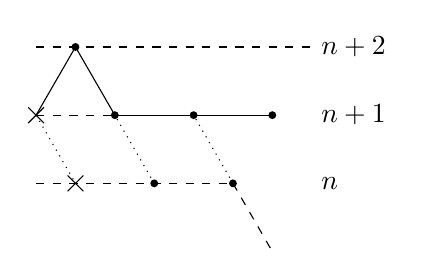
\begin{tikzpicture}
      \draw [dashed] (-0.5, 0.0) -- (2.0, 0.0);
      \fill (3.0, 0.0) node [right] {$n$};
      \draw [dashed] (-0.5, 0.866) -- (2.5, 0.866);
      \fill (3.0, 0.866) node [right] {$n+1$};
      \draw [dashed] (-0.5, 1.732) -- (3.0, 1.732);
      \fill (3.0, 1.732) node [right] {$n+2$};
      \fill (60 : 1.0) circle [radius = 0.05];
      \draw (-0.1,-0.1) -- (0.1,0.1);
      \draw (0.1,-0.1) -- (-0.1,0.1);
      \begin{scope}[shift = (120 : 1.0)]
        \draw (-0.1,-0.1) -- (0.1,0.1);
        \draw (0.1,-0.1) -- (-0.1,0.1);
      \end{scope}
      \begin{scope}[shift = (120 : 1.0)]
        \draw [dotted] (0 : 0.0) -- (300 : 1.0);
      \end{scope}
      \begin{scope}[shift = (60 : 1.0)]
        \draw (0.0, 0.0) -- (2.0, 0.0);
        \fill (2.0, 0.0) circle [radius = 0.05];
      \end{scope}
      \begin{scope}[shift = (0 : 2.0)]
        \draw [dashed] (0 : 0.0) -- (300 : 1.0);
      \end{scope}
      \begin{scope}[shift = (0 : 1.0)]
      \fill (0.0, 0.0) circle [radius = 0.05];
        \foreach \theta in {0, 60}{
          \fill (0,0) [transform canvas = {shift = (\theta : 1.0)}] circle [radius = 0.05];
        }
        \draw [dotted] (0 : 0.0) -- (120 : 1.0);
      \end{scope}
      \begin{scope}[shift = (0 : 2.0)]
        \draw [dotted] (0 : 0.0) -- (120 : 1.0);
      \end{scope}
      \begin{scope}[shift = (60 : 1.0)]
        \begin{scope}[shift = (120 : 1.0)]
          \fill (0.0, 0.0) circle [radius = 0.05];
          \draw (0 : 0.0) -- (240 : 1.0);
          \draw (0 : 0.0) -- (300 : 1.0);
        \end{scope}
      \end{scope}
    \end{tikzpicture}

    \begin{tikzpicture}
      \draw [dashed] (-0.5, 0.0) -- (2.0, 0.0);
      \fill (3.0, 0.0) node [right] {$n$};
      \draw [dashed] (-0.5, 0.866) -- (2.5, 0.866);
      \fill (3.0, 0.866) node [right] {$n+1$};
      \draw (-0.1,-0.1) -- (0.1,0.1);
      \draw (0.1,-0.1) -- (-0.1,0.1);
      \fill (60 : 1.0) circle [radius = 0.05];
      \begin{scope}[shift = (120 : 1.0)]
        \draw (-0.1,-0.1) -- (0.1,0.1);
        \draw (0.1,-0.1) -- (-0.1,0.1);
      \end{scope}
      \begin{scope}[shift = (120 : 1.0)]
        \draw [dotted] (0 : 0.0) -- (300 : 1.0);
        \draw (0.0, 0.0) -- (3.0, 0.0);
      \end{scope}
      \begin{scope}[shift = (0 : 2.0)]
        \draw [dashed] (0 : 0.0) -- (300 : 1.0);
        \fill (60 : 1.0) circle [radius = 0.05];
      \end{scope}
      \begin{scope}[shift = (0 : 1.0)]
        \fill (0.0, 0.0) circle [radius = 0.05];
        \foreach \theta in {0, 60}{
          \fill (0,0) [transform canvas = {shift = (\theta : 1.0)}] circle [radius = 0.05];
        }
        \draw [dotted] (0 : 0.0) -- (120 : 1.0);
      \end{scope}
      \begin{scope}[shift = (0 : 2.0)]
        \draw [dotted] (0 : 0.0) -- (120 : 1.0);
      \end{scope}
    \end{tikzpicture}
    \end{tabular}
    \caption{}
  \end{center}
\end{figure}

Then, we will discuss the moment after the first the is fixed on a side of an equilateral hexagon with a radius of $n+1$. Let us assume that the bead is able to make a hydrogen bond. If it is able to make only two hydrogen bonds, it will be nondeterministic because there are possibilities that it makes two structures in Fig.8. Hence, it needs to make three hydrogen bonds to determine the only structure. It needs to be a right or left figure in Fig.9. to make three hydrogen bonds.\\

\begin{figure}
  \begin{center}
  \begin{tabular}{cc}
    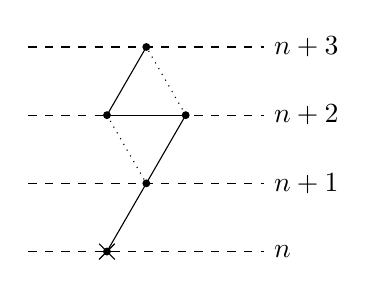
\begin{tikzpicture}
        \begin{scope}[shift=(0 : 0.0)]
          \draw (-0.1,-0.1) -- (0.1,0.1);
          \draw (0.1,-0.1) -- (-0.1,0.1);
          \draw (0 : 0.0) -- (60 : 1.0);
        \end{scope}
      \draw [dashed] (-1.0, 0.0) -- (2.0, 0.0);
      \fill (2.0, 0.0) node [right] {$n$};
      \draw [dashed] (-1.0, 0.866) -- (2.0, 0.866);
      \fill (2.0, 0.866) node [right] {$n+1$};
      \draw [dashed] (-1.0, 1.732) -- (2.0, 1.732);
      \fill (2.0, 1.732) node [right] {$n+2$};
      \draw [dashed] (-1.0, 2.598) -- (2.0, 2.598);
      \fill (2.0, 2.598) node [right] {$n+3$};
      \fill (0,0) circle [radius = 0.05];
      \begin{scope}[shift = (60 : 2.0)]
        \fill(0.0, 0.0) circle [radius = 0.05];
        \foreach \theta in {120, 180, 240}{
          \fill (0.0, 0.0) [transform canvas = {shift = (\theta : 1.0)}] circle [radius = 0.05];
        }
        \draw [dotted] (0 : 0.0) -- (120 : 1.0);
        \draw (0 : 0.0) -- (180 : 1.0);
        \draw (0 : 0.0) -- (240 : 1.0);
      \end{scope}
      \begin{scope}[shift = (60 : 1.0)]
        \begin{scope}[shift = (120 : 1.0)]
          \draw (0.0, 0.0) -- (60 : 1.0);
          \draw [dotted] (0.0, 0.0) -- (300 : 1.0);
        \end{scope}
      \end{scope}
    \end{tikzpicture}

    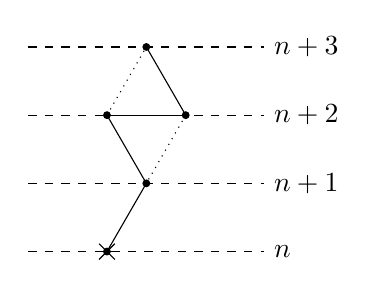
\begin{tikzpicture}
        \begin{scope}[shift=(0 : 0.0)]
          \draw (-0.1,-0.1) -- (0.1,0.1);
          \draw (0.1,-0.1) -- (-0.1,0.1);
          \draw (0 : 0.0) -- (60 : 1.0);
        \end{scope}
      \draw [dashed] (-1.0, 0.0) -- (2.0, 0.0);
      \fill (2.0, 0.0) node [right] {$n$};
      \draw [dashed] (-1.0, 0.866) -- (2.0, 0.866);
      \fill (2.0, 0.866) node [right] {$n+1$};
      \draw [dashed] (-1.0, 1.732) -- (2.0, 1.732);
      \fill (2.0, 1.732) node [right] {$n+2$};
      \draw [dashed] (-1.0, 2.598) -- (2.0, 2.598);
      \fill (2.0, 2.598) node [right] {$n+3$};
      \fill (0,0) circle [radius = 0.05];
      \begin{scope}[shift = (60 : 2.0)]
        \fill(0.0, 0.0) circle [radius = 0.05];
        \foreach \theta in {120, 180, 240}{
          \fill (0.0, 0.0) [transform canvas = {shift = (\theta : 1.0)}] circle [radius = 0.05];
        }
        \draw (0 : 0.0) -- (120 : 1.0);
        \draw (0 : 0.0) -- (180 : 1.0);
        \draw [dotted] (0 : 0.0) -- (240 : 1.0);
      \end{scope}
      \begin{scope}[shift = (60 : 1.0)]
        \begin{scope}[shift = (120 : 1.0)]
          \draw [dotted] (0.0, 0.0) -- (60 : 1.0);
          \draw (0.0, 0.0) -- (300 : 1.0);
        \end{scope}
      \end{scope}
    \end{tikzpicture}
    \end{tabular}
    \caption{}
  \end{center}
\end{figure}

 If it makes three hydrogen bonds once such as Fig.9., it will make three hyrogen bonds forever to be deterministic. This becomes nondeterministic finally, such as in Fig.7., when it reaches a corner of an equilateral hexagon. Therefore, the first fixed bead on a side of an equilateral hexagon with a radius of $n+1$ has to make a hydrogen bond with a molecule on a side of an equilateral hexagon with a radius of $n$.

\begin{figure}
  \begin{center}
  \begin{tabular}{cc}
    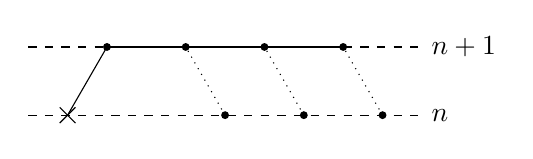
\begin{tikzpicture}
      \begin{scope}[shift=(0 : 0.0)]
        \draw (-0.1,-0.1) -- (0.1,0.1);
        \draw (0.1,-0.1) -- (-0.1,0.1);
        \draw (0 : 0.0) -- (60 : 1.0);
      \end{scope}
      \draw [dashed] (-0.5, 0.0) -- (4.5, 0.0);
      \fill (4.5, 0.0) node [right] {$n$};
      \draw [dashed] (-0.5, 0.866) -- (4.5, 0.866);
      \fill (4.5, 0.866) node [right] {$n+1$};
      \fill (2.0, 0.0) circle [radius = 0.05];
      \fill (3.0, 0.0) circle [radius = 0.05];
      \fill (4.0, 0.0) circle [radius = 0.05];
      \begin{scope}[shift = (60 : 1.0)]
        \fill (0.0, 0.0) circle [radius = 0.05];
        \fill (1.0, 0.0) circle [radius = 0.05];
        \fill (2.0, 0.0) circle [radius = 0.05];
        \fill (3.0, 0.0) circle [radius = 0.05];
        \draw (0.0, 0.0) -- (3.0, 0.0);
      \end{scope}
      \begin{scope}[shift = (0 : 2.0)]
        \draw [dotted] (0 : 0.0) -- (120 : 1.0);
      \end{scope}
      \begin{scope}[shift = (0 : 3.0)]
        \draw [dotted] (0 : 0.0) -- (120 : 1.0);
      \end{scope}
      \begin{scope}[shift = (0 : 4.0)]
        \draw [dotted] (0 : 0.0) -- (120 : 1.0);
      \end{scope}
    \end{tikzpicture}

    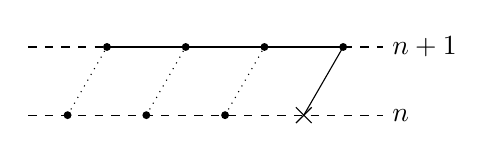
\begin{tikzpicture}
      \begin{scope}[shift=(0 : 0.0)]
        \draw (-0.1,-0.1) -- (0.1,0.1);
        \draw (0.1,-0.1) -- (-0.1,0.1);
        \draw (0 : 0.0) -- (60 : 1.0);
      \end{scope}
      \draw [dashed] (-3.5, 0.0) -- (1.0, 0.0);
      \fill (1.0, 0.0) node [right] {$n$};
      \draw [dashed] (-3.5, 0.866) -- (1.0, 0.866);
      \fill (1.0, 0.866) node [right] {$n+1$};
      \fill (-1.0, 0.0) circle [radius = 0.05];
      \fill (-2.0, 0.0) circle [radius = 0.05];
      \fill (-3.0, 0.0) circle [radius = 0.05];
      \begin{scope}[shift = (60 : 1.0)]
        \fill (0.0, 0.0) circle [radius = 0.05];
        \fill (-1.0, 0.0) circle [radius = 0.05];
        \fill (-2.0, 0.0) circle [radius = 0.05];
        \fill (-3.0, 0.0) circle [radius = 0.05];
        \draw (0.0, 0.0) -- (-3.0, 0.0);
      \end{scope}
      \begin{scope}[shift = (0 : -1.0)]
        \draw [dotted] (0 : 0.0) -- (60 : 1.0);
      \end{scope}
      \begin{scope}[shift = (0 : -2.0)]
        \draw [dotted] (0 : 0.0) -- (60 : 1.0);
      \end{scope}
      \begin{scope}[shift = (0 : -3.0)]
        \draw [dotted] (0 : 0.0) -- (60 : 1.0);
      \end{scope}
    \end{tikzpicture}
    \end{tabular}
    \caption{}
  \end{center}
\end{figure}

Accordingly, it is Fig.10. when a first bead is fixed on a side of an equilateral hexagon with a radius of $n+1$.

\begin{figure}
  \begin{center}
    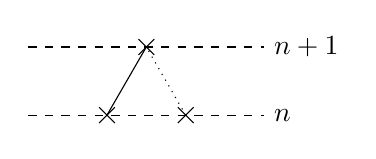
\begin{tikzpicture}
      \draw [dashed] (-1.0, 0.0) -- (2.0, 0.0);
      \fill (2.0, 0.0) node [right] {$n$};
      \draw [dashed] (-1.0, 0.866) -- (2.0, 0.866);
      \fill (2.0, 0.866) node [right] {$n+1$};
      \begin{scope}[shift=(0 : 0.0)]
        \draw (-0.1,-0.1) -- (0.1,0.1);
        \draw (0.1,-0.1) -- (-0.1,0.1);
        \draw (0 : 0.0) -- (60 : 1.0);
      \end{scope}
      \begin{scope}[shift=(60 : 1.0)]
        \draw (-0.1,-0.1) -- (0.1,0.1);
        \draw (0.1,-0.1) -- (-0.1,0.1);
      \end{scope}
      \begin{scope}[shift=(0 : 1.0)]
        \draw (-0.1,-0.1) -- (0.1,0.1);
        \draw (0.1,-0.1) -- (-0.1,0.1);
        \draw [dotted] (0 : 0.0) -- (120 : 1.0);
      \end{scope}
    \end{tikzpicture}
    \caption{}
  \end{center}
\end{figure}

It has to be a right or left figure in Fig.6. when the first bead fixed on a side of an equilateral hexagon with a radius of $n+1$ make a hydrogen bond with a bead on a side of an equilateral hexagon with a radius of $n$. Fig.6. becomes nondeterministic finally, such as in Fig.7., when it reaches a corner of an equilateral hexagon. It is clear that all beads on a side of an equilateral hexagon with a radius of $n+1$ has to make a hydrogen bond with a bead on a side of an equilateral hexagon with a radius of $n$.  It is impossible to fix molecules on a side of an equilateral hexagon with a radius of $n+2$ and determine the only structure when there are only beads which are able to make a hydrogen bond in an equilateral hexagon with a radius of $n$.
